\documentclass[aspectratio=169, 10pt]{beamer}

\usepackage{bm} % bold math
\usepackage{fontspec}
\usepackage{minted}
\usepackage{pgf-pie}
\usepackage{tikz}
\usepackage{graphicx}
\newcommand\sbullet[1][.5]{\mathbin{\vcenter{\hbox{\scalebox{#1}{$\bullet$}}}}}

% Custom commands and environments
\makeatletter
\newcommand\version[1]{\renewcommand\@version{#1}}
\newcommand\@version{}
\def\insertversion{\@version}

\newcommand\course[1]{\renewcommand\@course{#1}}
\newcommand\@course{}
\def\insertcourse{\@course}

\newcommand\coursetitle[1]{\renewcommand\@coursetitle{#1}}
\newcommand\@coursetitle{}
\def\insertcoursetitle{\@coursetitle}

\newcommand\lecturenumber[1]{\renewcommand\@lecturenumber{#1}}
\newcommand\@lecturenumber{}
\def\insertlecturenumber{\@lecturenumber}
\makeatother

\newcommand{\slidetitle}[1]{{\xbseries \large \structure{#1}} \bigskip}
\newcommand{\term}[1]{{\color{blue} #1}}
\newcommand{\leftspace}{\hspace{1em}}
\newcommand{\inlinearrow}{
  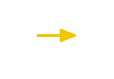
\begin{tikzpicture}[baseline]
    \node [anchor=base] (x) {};
    \draw [rawarrow] (x.mid west) -- ($(x.mid west) + (2em,0)$);
  \end{tikzpicture}
}

\newenvironment{slide}
{\begin{frame}[fragile,environment=slide]\vskip0pt plus 1filll}
{\vskip0pt plus 1filll\end{frame}}

% LaTeX

\setlength{\leftmargini}{1em}

% Common Information

\author{Talia Xu}
\course{COMPSCI 340}
\coursetitle{Operating Systems}
\date{2024 Semester 2}

% fontspec

\defaultfontfeatures{Ligatures=TeX}
% \setmainfont{Domine}
\setsansfont{Inter}[
  FontFace={ul}{n}{Font=*-Thin},
  FontFace={el}{n}{Font=*-ExtraLight},
  FontFace={l}{n}{Font=*-Light},
  FontFace={sb}{n}{Font=*-SemiBold},
  FontFace={eb}{n}{Font=*-ExtraBold},
  FontFace={xb}{n}{Font=*-Black},
]
\setmonofont[Contextuals=AlternateOff, Ligatures=TeXOff]{Iosevka}[
  FontFace={xb}{n}{Font=*-Heavy},
]

%% Font Weights

\DeclareRobustCommand{\ulseries}{\fontseries{ul}\selectfont}
\DeclareTextFontCommand{\textul}{\ulseries}
\DeclareRobustCommand{\elseries}{\fontseries{el}\selectfont}
\DeclareTextFontCommand{\textel}{\elseries}
\DeclareRobustCommand{\lseries}{\fontseries{l}\selectfont}
\DeclareTextFontCommand{\textl}{\lseries}
\DeclareRobustCommand{\sbseries}{\fontseries{sb}\selectfont}
\DeclareTextFontCommand{\textsb}{\sbseries}
\DeclareRobustCommand{\ebseries}{\fontseries{eb}\selectfont}
\DeclareTextFontCommand{\texteb}{\ebseries}
\DeclareRobustCommand{\xbseries}{\fontseries{xb}\selectfont}
\DeclareTextFontCommand{\textxb}{\xbseries}

% tikz

\usetikzlibrary{
  arrows,
  arrows.meta,
  automata,
  backgrounds,
  calc,
  decorations.pathreplacing,
  matrix,
  positioning,
  overlay-beamer-styles,
  shapes,
  shapes.multipart,
  tikzmark,
}

\tikzstyle{rawarrow} = [
  -{Latex[round]},
  line width=1pt,
  yellow,
  shorten >=3pt,
  shorten <=3pt,
  font=\small,
  text=black,
]

\tikzstyle{arrow} = [
  -{Latex[round]},
  line width=1pt,
  yellow,
  shorten >=3pt,
  shorten <=3pt,
  transform canvas={yshift=3pt},
  font=\small,
  text=black,
]

\newcommand{\tikzmarkcoord}[1]{([yshift=3pt]pic cs:#1)}

% minted

\setminted{style=eyolfson, fontsize=\small, escapeinside=||}
\setmintedinline{fontsize=\normalsize}

% hyperref

\hypersetup{colorlinks, urlcolor=blue}

% beamer
\setbeamersize{text margin left=16mm, text margin right=16mm}
\setbeamertemplate{itemize items}[circle]
\setbeamercolor{item}{fg=black}
\setbeamercolor{structure}{fg=darkblue}
\setbeamerfont{frametitle}{series=\bfseries, parent=structure}
\setbeamertemplate{navigation symbols}{}
\setbeamertemplate{headline}{}
\setbeamertemplate{footline}{
  \begin{tikzpicture}[
    remember picture,
    overlay,
    shift={(current page.south west)},
  ]
    \path [fill=gray] (144mm, 0) -- (160mm, 16mm) -- (160mm, 0);
    \node [inner sep=3.5mm, outer sep=0, text=black, anchor=base east,
           align=right, yshift=3.5mm]
          at (current page.south east) {\ttfamily \small \insertframenumber{}};
  \end{tikzpicture}
}
\setbeamertemplate{title page}{
  \begin{tikzpicture}[
    remember picture,
    overlay,
    shift={(current page.south west)},
    background rectangle/.style={fill=darkblue},
    show background rectangle,
  ]
    \node [anchor=center, align=center, text=white, text width=40mm, scale=3.2]
          at (\paperwidth / 2, \paperheight * 2 / 3)
          {\xbseries \inserttitle{}};
    \node [anchor=base west, align=left, inner sep=0, text=white, yshift=2.5mm]
          at (16mm, \paperheight / 3)
          {\insertdate{} \insertcourse{}: \insertcoursetitle{}};
    \node [anchor=base west, align=left, inner sep=0, text=white, yshift=-2.5mm]
          at (16mm, \paperheight / 3)
          {\insertauthor};
    \node [anchor=base east, align=right, inner sep=0, text=white, yshift=2.5mm]
          at (144mm, \paperheight / 3)
          {Lecture \insertlecturenumber{}};
    \node [anchor=base east, align=right, inner sep=0, text=white,
           yshift=-2.5mm]
          at (144mm, \paperheight / 3)
          {\ttfamily \insertversion{}};
    \node [align=center, anchor=south, inner sep=0, text=white, yshift=3.5mm]
          (license) at (\paperwidth / 2, 0)
          {\fontsize{7pt}{7pt}\selectfont This  work is licensed under a
           \href{http://creativecommons.org/licenses/by-sa/4.0/}
                {\color{lightblue} Creative Commons Attribution-ShareAlike 4.0
                 International License}};
  \end{tikzpicture}
}

% xcolor

%% Primary Colour

\definecolor{pantone655}{RGB}{0, 42, 92} % #002a5c
\colorlet{darkblue}{pantone655}

%% Secondary Colours

\definecolor{pantone633}{RGB}{0, 139, 176} % #008bb0
\colorlet{blue}{pantone633}

\definecolor{pantonewarmred}{RGB}{220, 70, 51} % #dc4633
\colorlet{red}{pantonewarmred}

\definecolor{pantone3285}{RGB}{0, 161, 137} % #00a189
\colorlet{cyan}{pantone3285}

\definecolor{pantone7722}{RGB}{13, 83, 77} % #0d534d
\colorlet{darkcyan}{pantone7722}

\definecolor{pantone376}{RGB}{141, 191, 46} % #8dbf2e
\colorlet{green}{pantone376}

\definecolor{pantone2613}{RGB}{109, 36, 122} % #6d247a
\colorlet{violet}{pantone2613}

\definecolor{pantone2985}{RGB}{111, 199, 234} % #6fc7ea
\colorlet{lightblue}{pantone2985}

\definecolor{pantone227}{RGB}{171, 19, 104} % #ab1368
\colorlet{magenta}{pantone227}

\definecolor{pantone7406}{RGB}{241, 197, 0} % #f1c500
\colorlet{yellow}{pantone7406}

%% Neutrals

\definecolor{pantonecoolgray2}{RGB}{208, 209, 201} % #d0d1c9
\colorlet{gray}{pantonecoolgray2}


\lecturenumber{19} 
\title{File\\Systems}
\version{1.0.0}

\begin{document}

\begin{slide}
	Please sit close to the front of the class to help me save my voice =)
	\bigskip
	
	Please sit close to someone if possible for in-class discussions.
\end{slide}

\begin{frame}[plain, noframenumbering]
    \titlepage
\end{frame}

\begin{slide}

    \slidetitle{I'm Talia, your instructor}
	
    I am a lecturer in the Computer Systems Group.
    \bigskip

    I am about to receive my PhD from TU Delft.
    \bigskip

   I previously went to University of Toronto for BASc and MASc.

\end{slide}

\begin{slide}

    \slidetitle{I'm Talia, your instructor}

    I worked at a few industry places, mostly as an intern 
    \begin{itemize}
    	\item Canada: IBM, Arista Networks, Amazon
	\item US: Reach Power (startup)
	\item UK: Nokia Bell Labs
    \end{itemize}

    \bigskip
    My research interest is 
    \begin{itemize}
	\item Using light for communication and sensing
	\item Novel sensing systems for health / mental well-beings
	\item Generally involvesome hardware or embedded systems
    \end{itemize}

\end{slide}

\begin{slide}

    \slidetitle{I'm Talia, your instructor}

    Office: 303s-592
    \bigskip

    Office hours: Monday 1 pm - 2 pm \& Friday 1 pm - 2 pm
    \bigskip

    Email: talia.xu@auckland.ac.nz

\end{slide}

\begin{slide}

    \slidetitle{Please provide feedback}

    Let me know what you like, dislike, or want to see more of
    \bigskip
    
    I'm open to suggestions!
	\bigskip
	
	Feedback through Discord: mtxu

\end{slide}

\begin{slide}

	\slidetitle{Acknowledgement}
	
	The slide template and content are built on materials from 
	\bigskip
	
	Professor Jon Eyolfson
	\medskip
	
	Professor  Paul Krzyzanowski
	\medskip
	
\end{slide}

\begin{slide}

    \slidetitle{These books complement lectures}

    ``\href{https://pages.cs.wisc.edu/~remzi/OSTEP/}
	   {Operating Systems: Three Easy Pieces}'' \\
    by \href{http://www.cs.wisc.edu/~remzi/}{Remzi Arpaci-Dusseau}
    and \href{http://www.cs.wisc.edu/~dusseau/}{Andrea Arpaci-Dusseau}
    \bigskip

    ``\href{https://en.wikipedia.org/wiki/Modern_Operating_Systems}
           {Modern Operating Systems}'' \\
    by \href{https://en.wikipedia.org/wiki/Andrew_S._Tanenbaum}{Andrew S. Tanenbaum}
    \bigskip
							      
    Test: You are only responsible for what have been covered in class.

\end{slide}

\begin{slide}

	\slidetitle{We will cover the following topics}
	
	File Systems
	\bigskip

	Distributed File Systems \& Distributed Systems
	\bigskip
	
	Memory
	\bigskip
	
	Security
	\bigskip
	
	(if time permits) Device Drivers

\end{slide}

\begin{slide}

    \slidetitle{Why should we care about OS?}

    \href{https://youtu.be/9lBbqH_1KS4?feature=shared}
           {Distinguished Lecture by Amin Vahdat}
    \bigskip

    \begin{itemize}
        \item \textbf{End of Moore's Law:} The traditional approach of relying on exponential hardware improvement is no longer sustainable.
        \item \textbf{Shifting Demands:} The growing demand for machine learning and data processing requires a different approach to computing infrastructure.
        \item \textbf{System-Level Optimization:} Optimizing the entire system, rather than individual components, can unlock greater gains in capacity and capability.
    \end{itemize}

\end{slide}

\begin{slide}

    \slidetitle{File System: How to manage a persistent device?}

    What are the APIs?
    \bigskip

    What are the important aspects of the implementation?

\end{slide}

%\begin{slide}
%
    % \slidetitle{File system: How to manage a persistent device?}

    % You have a 1 MB file named \textbf{foo} stored in the directory \textbf{/bar}
    % \begin{itemize}
        % \item What is the \textbf{full path name} of foo?
		% \item Your working directory is /bar, what is the \textbf{relative path name} of foo?
		% \item Your working directory is /bar/sbar, what is the \textbf{relative path name} of foo?
    % \end{itemize}
% \end{slide}

% \begin{slide}

	% \slidetitle{File system: How to manage a persistent device?}

    % You have a 1 MB file named \textbf{foo} stored in the directory \textbf{/bar}
    % \begin{itemize}
        % \item What is the \textbf{full path name} of foo?
		% \item You are in the directory /bar, what is the \textbf{relative path name} of foo?
		% \item You are in a subdirectory /bar/sbar, what is the \textbf{relative path name} of foo?
    % \end{itemize}
	% \bigskip
	
	% What happens in the file system when you enter a path name to retrieve a file?
	% \bigskip
	
	% Can you create a flowchart to illustrate this process?
% \end{slide}

\begin{slide}

	\slidetitle{File system: How to manage a persistent device?}

    How are files organized on the disk? 
    \begin{itemize}
        \item What \textbf{data structures} are used to store the data of the file?
        \item The \textbf{metadata}?
        \item The \textbf{location}?
    \end{itemize}
    \bigskip

    How do you access data on the disk?
    \begin{itemize}
        \item When you open/write/read the file, what \textbf{function calls} are evoked?
        \item If we write another 1MB data to /bar/foo, where does this data go?
        \item Which structures on the disks are read from and written to?
    \end{itemize}

\end{slide}

\begin{slide}

    \slidetitle{File system is an abstract concept}

    A File system describes a way of organizing and storing files on a storage device.

    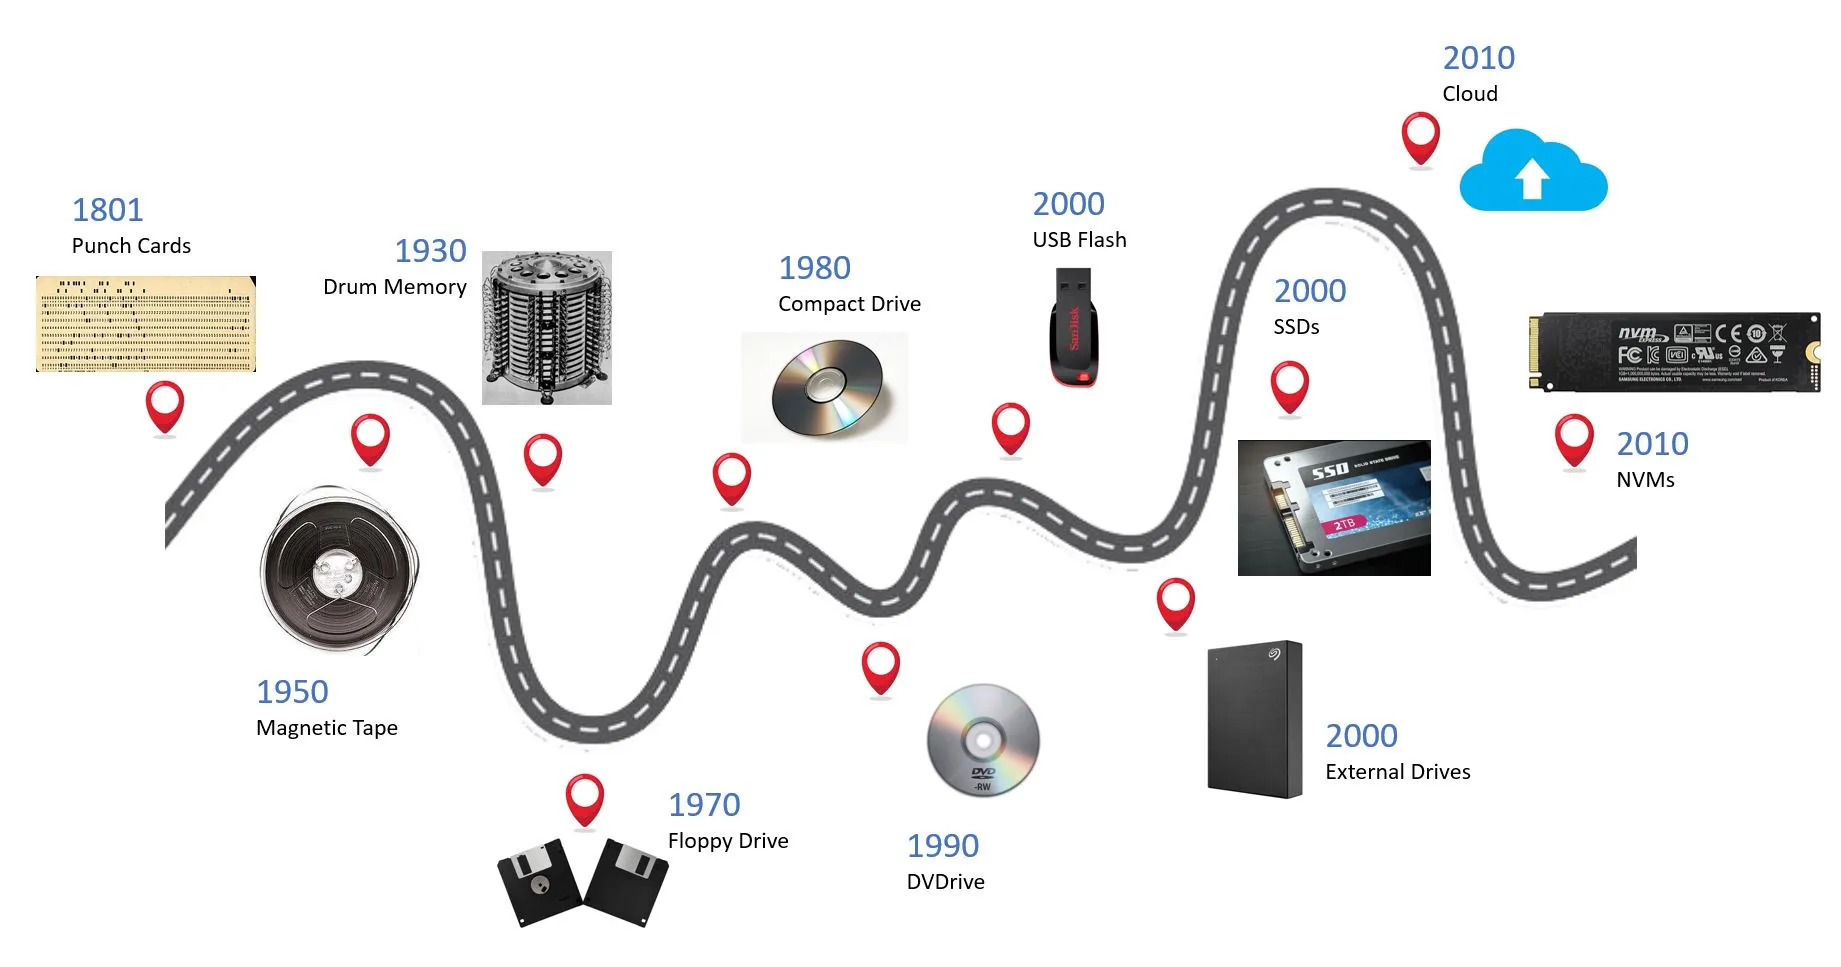
\includegraphics[width=64mm]{file-system-hardware.jpg}
    
    What are some requirements of a file system?
    \begin{itemize}
        \item \textbf{Availability:} Ensure data can be accessed and used reliably.
        \item \textbf{Permanence:} Store data permanently (or an approximation of it).
        \item \textbf{Concurrent Access:} Make data sharable with other programs or users
    \end{itemize}

\end{slide}

\begin{slide}

    \slidetitle{File system implementations are design choices}

	\begin{minipage}{0.45\textwidth}
        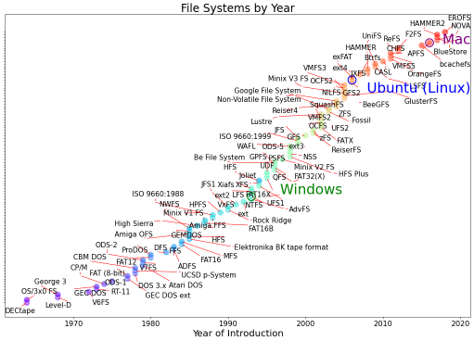
\includegraphics[width=54mm]{file-system-implementation.png}
    \end{minipage}
    \hfill
    \begin{minipage}{0.52\textwidth}
		Performance (Speed) is also important.
		\bigskip
		
		Performance is application specific.
		\bigskip
		
		Some popular file system implementations: 
		\begin{itemize}
			\item Unix (Linux and Mac)
			\item Windows
			\item Specialized system (Mainframe)
		\end{itemize}
    \end{minipage}
	    
\end{slide}

\begin{slide}

    \slidetitle{What is a file?}

    Textbook: A named collection of related information that is recorded on secondary storage.
    \bigskip

    For most users, the basic unit of interaction with a file system is a file.
    \bigskip

    \begin{itemize}
        \item Is a directory a file?
        \item Is a process a file?
        \item Is a device a file?
    \end{itemize}

\end{slide}

\begin{slide}
    
    \slidetitle{Usual layout of a POSIX Filesystem}

    POSIX is a set of standards that provides a common interface for operating systems.
  

    \begin{center}
        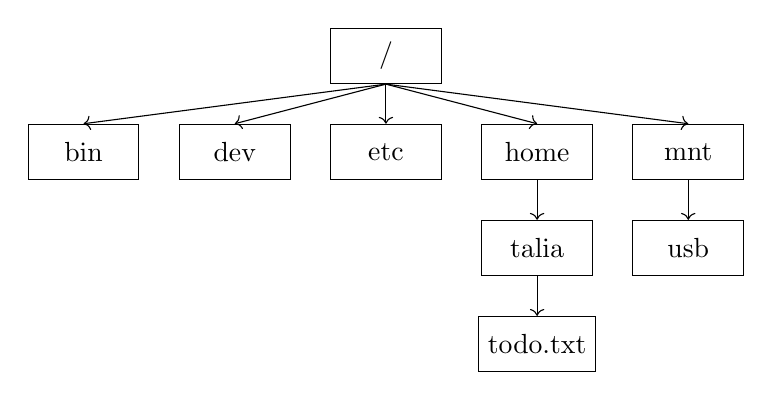
\begin{tikzpicture}[node distance=-2mm and 5mm]

        \node[draw,rectangle,minimum width=40,minimum height=20] (root)  {/};
        \node[draw,rectangle,minimum width=40,minimum height=20,yshift=-20] (etc) [below=of root] {etc};
        \node[draw,rectangle,minimum width=40,minimum height=20] (dev) [left=of etc] {dev};
        \node[draw,rectangle,minimum width=40,minimum height=20] (bin) [left=of dev] {bin};
        \node[draw,rectangle,minimum width=40,minimum height=20] (home) [right=of etc] {home};
        \node[draw,rectangle,minimum width=40,minimum height=20] (mnt) [right=of home] {mnt};
    
        \node[draw,rectangle,minimum width=40,minimum height=20,yshift=-20] (talia) [below=of home] {talia};
        \node[draw,rectangle,minimum width=40,minimum height=20,yshift=-20] (todotxt) [below=of talia] {todo.txt};
    
        \node[draw,rectangle,minimum width=40,minimum height=20,yshift=-20] (usb) [below=of mnt] {usb};
    
        \draw[->] (root.south) -- (bin.north);
        \draw[->] (root.south) -- (dev.north);
        \draw[->] (root.south) -- (etc.north);
        \draw[->] (root.south) -- (home.north);
        \draw[->] (root.south) -- (mnt.north);
        \draw[->] (home.south) -- (talia.north);
        \draw[->] (mnt.south) -- (usb.north);
        \draw[->] (talia.south) -- (todotxt.north);
    
        \end{tikzpicture}
    \end{center}

    Working Directory: /home/talia
    \begin{itemize}
        \item What is the absolute and relative path to \textbf{todo.txt}?
              To \textbf{usb}?
    \end{itemize}

\end{slide}
  
\begin{slide}
    
    \slidetitle{POSIX Filesystem}

    todo.txt Relative: ./todo.txt

    todo.txt Absolute: /home/jon/todo.txt

    usb Relative: ../../mnt/usb

    usb Absolute: /mnt/usb
    \bigskip

    Special symbols:

    \leftspace{}. --- Current directory
    
    \leftspace{}.. ---  Parent directory

    \leftspace{}$\mathsf{\sim}$ --- User's home directory (\$HOME)
    \bigskip

    Relative paths are calculated from current working directory (\$PWD)

\end{slide}

\begin{slide}
    
    \slidetitle{You Can Access Files Sequentially or Randomly}

    \textbf{Sequential access}
    \begin{itemize}
        \item Each read advances the position inside the file
        \item Writes are appended and the position set to the end afterwards
    \end{itemize}
	\bigskip

    \textbf{Random access}
    \begin{itemize}
        \item Records can be read/written to the file in any order
        \item A specific position is required for each operation
    \end{itemize}

\end{slide}

\begin{slide}
    
    \slidetitle{POSIX Filesystem}

    \begin{minted}{c}
int open(const char *pathname, int flags, mode_t mode);

// flags can specify which operations: O_RDWR,O_WRONLY, O_RDWR
// also: O_APPEND moves the position to the end of the file initially

off_t lseek(int fd, off_t offset, int whence);

// lseek changes the position to the offset
// whence can be one of: SEEK_SET, SEEK_CUR, SEEK_END
//   set makes the offset absolute, cur and end are both relative
  \end{minted}

\end{slide}
  
\begin{slide}
    
    \slidetitle{File Tables Are Stored in the Process Control Block (PCB)}

    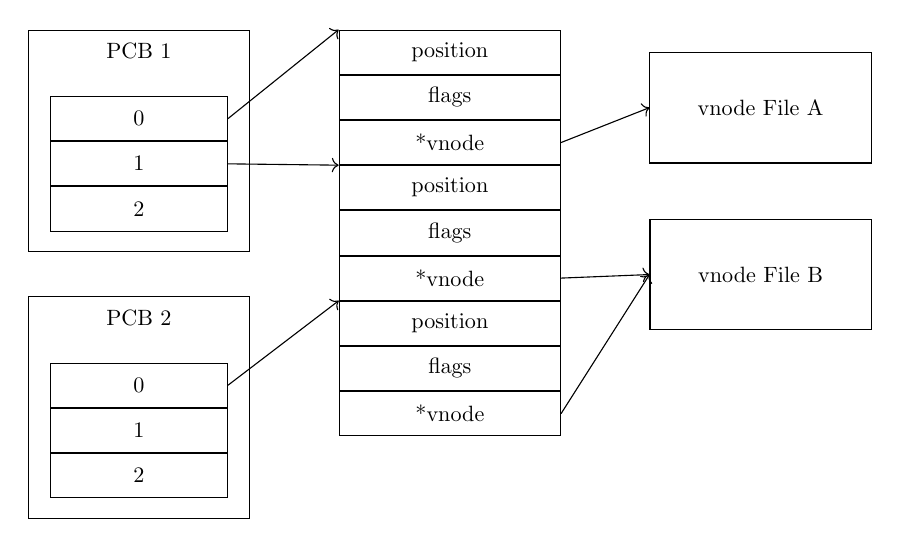
\begin{tikzpicture}[node distance=0mm and 0mm,scale=0.8, every node/.style={transform shape}]
      \node[rectangle,draw,minimum width=100,minimum height=100] (pcb1)      {};
      \node[rectangle,minimum width=100,minimum height=20,yshift=-20] (pcb11) [above=of pcb1] {PCB 1};
      \node[rectangle,draw,minimum width=80,minimum height=20,xshift=0,yshift=-10] (lof11) [below=of pcb11] {0};
      \node[rectangle,draw,minimum width=80,minimum height=20] (lof12) [below=of lof11] {1};
      \node[rectangle,draw,minimum width=80,minimum height=20] (lof13) [below=of lof12] {2};


      \node[rectangle,draw,minimum width=100,minimum height=100,yshift=-20] (pcb2)   [below=of pcb1]   {};
      \node[rectangle,minimum width=100,minimum height=20,yshift=-20] (pcb21) [above=of pcb2] {PCB 2};
      \node[rectangle,draw,minimum width=80,minimum height=20,xshift=0,yshift=-10] (lof21) [below=of pcb21] {0};
      \node[rectangle,draw,minimum width=80,minimum height=20] (lof22) [below=of lof21] {1};
      \node[rectangle,draw,minimum width=80,minimum height=20] (lof23) [below=of lof22] {2};

      \node[rectangle,draw,minimum width=100,minimum height=20,xshift=40,yshift=40] (gof1)   [right=of pcb1]   {position};
      \node[rectangle,draw,minimum width=100,minimum height=20] (gof2)   [below=of gof1]   {flags};
      \node[rectangle,draw,minimum width=100,minimum height=20] (gof3)   [below=of gof2]   {*vnode};

      \node[rectangle,draw,minimum width=100,minimum height=20] (gof4)   [below=of gof3]   {position};
      \node[rectangle,draw,minimum width=100,minimum height=20] (gof5)   [below=of gof4]   {flags};
      \node[rectangle,draw,minimum width=100,minimum height=20] (gof6)   [below=of gof5]   {*vnode};

      \node[rectangle,draw,minimum width=100,minimum height=20] (gof7)   [below=of gof6]   {position};
      \node[rectangle,draw,minimum width=100,minimum height=20] (gof8)   [below=of gof7]   {flags};
      \node[rectangle,draw,minimum width=100,minimum height=20] (gof9)   [below=of gof8]   {*vnode};

      \node[rectangle,draw,minimum width=100,minimum height=50,xshift=40,yshift=-25] (vnode1)  [right=of gof1]    {vnode File A};
      \node[rectangle,draw,minimum width=100,minimum height=50,yshift=-25] (vnode2)  [below=of vnode1]    {vnode File B};

      \draw[->] (lof11.east) -- (gof1.north west);
      \draw[->] (lof12.east) -- (gof4.north west);
      \draw[->] (lof21.east) -- (gof7.north west);

      \draw[->] (gof3.east) -- (vnode1.west);
      \draw[->] (gof6.east) -- (vnode2.west);
      \draw[->] (gof9.east) -- (vnode2.west);        
    \end{tikzpicture}
	
\end{slide}
  
 \begin{slide}
    
    \slidetitle{Each Process Contains a File Table in its PCB}

     A \textbf{Fie Descriptor} is an \textbf{index} in the table
    \bigskip

     Each item points to a system-wide \textit{global open file \textbf{(GOF)} table}
    \bigskip

     The GOF table holds information about the \textbf{seek position} and \textbf{flags}
	\begin{itemize}
		\item It also points to a \textit{VNode} (supports read/write/etc)
	\end{itemize}
    \bigskip

     A \textbf{vnode} (virtual mode) holds information about the file
	\begin{itemize}
	    \item vnodes can represent regular files, pipes, network sockets, etc.
	\end{itemize}

 \end{slide}

 \begin{slide}
    
    \slidetitle{What happens in a fork?}

    PCB is copied – local open file table gets inherited
	\bigskip
	
	Both PCBs point to the same Global Open Table entry

 \end{slide}

 \begin{slide}
    
    \slidetitle{Both Processes Point to the Same GOF Entry}

    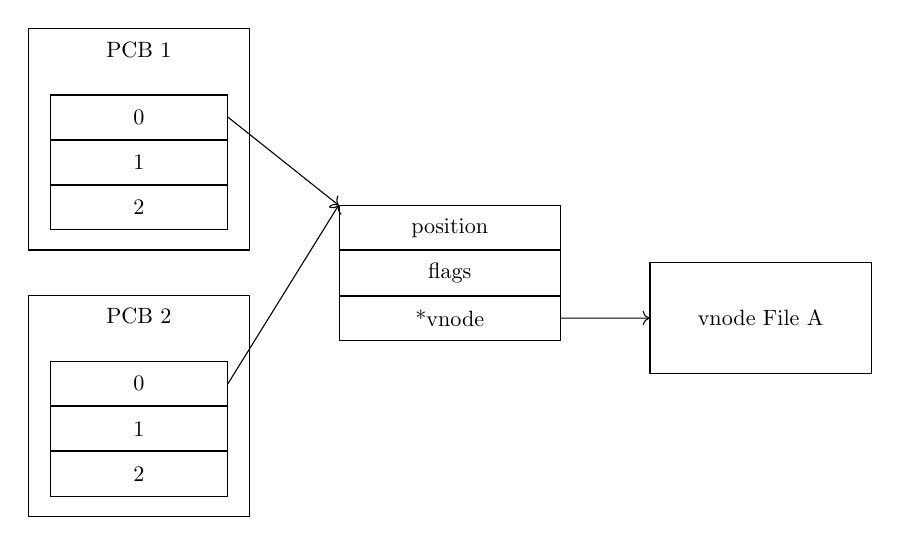
\begin{tikzpicture}[node distance=0mm and 0mm,scale=0.8, every node/.style={transform shape}]
      
      \node[rectangle,draw,minimum width=100,minimum height=100] (pcb1)      {};
      \node[rectangle,minimum width=100,minimum height=20,yshift=-20] (pcb11) [above=of pcb1] {PCB 1};
      \node[rectangle,draw,minimum width=80,minimum height=20,xshift=0,yshift=-10] (lof11) [below=of pcb11] {0};
      \node[rectangle,draw,minimum width=80,minimum height=20] (lof12) [below=of lof11] {1};
      \node[rectangle,draw,minimum width=80,minimum height=20] (lof13) [below=of lof12] {2};


      \node[rectangle,draw,minimum width=100,minimum height=100,yshift=-20] (pcb2)   [below=of pcb1]   {};
      \node[rectangle,minimum width=100,minimum height=20,yshift=-20] (pcb21) [above=of pcb2] {PCB 2};
      \node[rectangle,draw,minimum width=80,minimum height=20,xshift=0,yshift=-10] (lof21) [below=of pcb21] {0};
      \node[rectangle,draw,minimum width=80,minimum height=20] (lof22) [below=of lof21] {1};
      \node[rectangle,draw,minimum width=80,minimum height=20] (lof23) [below=of lof22] {2};

      \node[rectangle,draw,minimum width=100,minimum height=20,xshift=40,yshift=-40] (gof1)   [right=of pcb1]   {position};
      \node[rectangle,draw,minimum width=100,minimum height=20] (gof2)   [below=of gof1]   {flags};
      \node[rectangle,draw,minimum width=100,minimum height=20] (gof3)   [below=of gof2]   {*vnode};

      \node[rectangle,draw,minimum width=100,minimum height=50,xshift=40] (vnode1)  [right=of gof3]    {vnode File A};

      \draw[->] (lof11.east) -- (gof1.north west);
      \draw[->] (lof21.east) -- (gof1.north west);

      \draw[->] (gof3.east) -- (vnode1.west);    

    \end{tikzpicture}

\end{slide}

\begin{slide}
    
    \slidetitle{How many LOF and GOF Entries Exist? What is the Relationship?}

    \begin{minted}{c}
open("todo.txt", O_RDONLY);
fork();
open("b.txt", O_RDONLY);
    \end{minted}
    \medskip

    Assume there are no previously opened files (not even the standard ones)

 \end{slide}

 \begin{slide}
    
    \slidetitle{There are 2 LOF Entries Each, and 3 GOF Entries}

    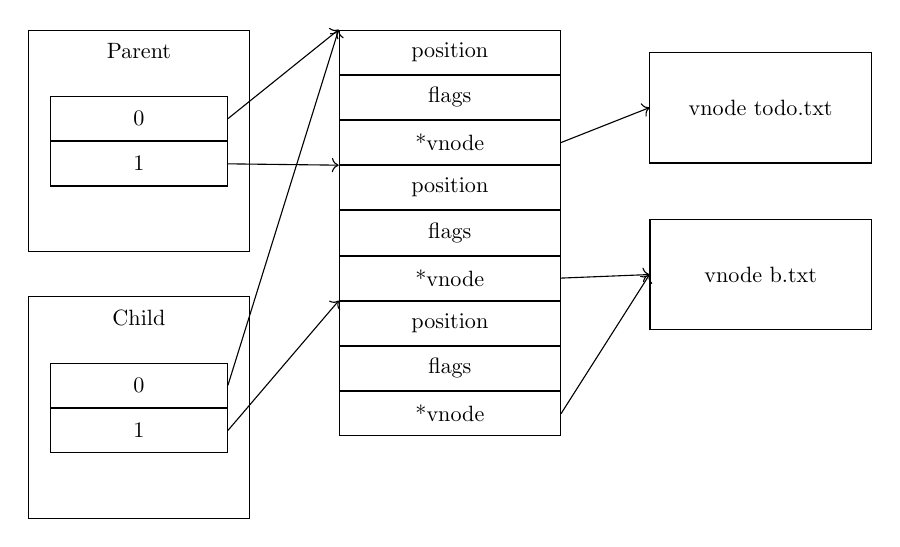
\begin{tikzpicture}[node distance=0mm and 0mm,scale=0.8, every node/.style={transform shape}]
        
      \node[rectangle,draw,minimum width=100,minimum height=100] (pcb1)      {};
      \node[rectangle,minimum width=100,minimum height=20,yshift=-20] (pcb11) [above=of pcb1] {Parent};
      \node[rectangle,draw,minimum width=80,minimum height=20,xshift=0,yshift=-10] (lof11) [below=of pcb11] {0};
      \node[rectangle,draw,minimum width=80,minimum height=20] (lof12) [below=of lof11] {1};


      \node[rectangle,draw,minimum width=100,minimum height=100,yshift=-20] (pcb2)   [below=of pcb1]   {};
      \node[rectangle,minimum width=100,minimum height=20,yshift=-20] (pcb21) [above=of pcb2] {Child};
      \node[rectangle,draw,minimum width=80,minimum height=20,xshift=0,yshift=-10] (lof21) [below=of pcb21] {0};
      \node[rectangle,draw,minimum width=80,minimum height=20] (lof22) [below=of lof21] {1};

      \node[rectangle,draw,minimum width=100,minimum height=20,xshift=40,yshift=40] (gof1)   [right=of pcb1]   {position};
      \node[rectangle,draw,minimum width=100,minimum height=20] (gof2)   [below=of gof1]   {flags};
      \node[rectangle,draw,minimum width=100,minimum height=20] (gof3)   [below=of gof2]   {*vnode};

      \node[rectangle,draw,minimum width=100,minimum height=20] (gof4)   [below=of gof3]   {position};
      \node[rectangle,draw,minimum width=100,minimum height=20] (gof5)   [below=of gof4]   {flags};
      \node[rectangle,draw,minimum width=100,minimum height=20] (gof6)   [below=of gof5]   {*vnode};

      \node[rectangle,draw,minimum width=100,minimum height=20] (gof7)   [below=of gof6]   {position};
      \node[rectangle,draw,minimum width=100,minimum height=20] (gof8)   [below=of gof7]   {flags};
      \node[rectangle,draw,minimum width=100,minimum height=20] (gof9)   [below=of gof8]   {*vnode};

      \node[rectangle,draw,minimum width=100,minimum height=50,xshift=40,yshift=-25] (vnode1)  [right=of gof1]    {vnode todo.txt};
      \node[rectangle,draw,minimum width=100,minimum height=50,yshift=-25] (vnode2)  [below=of vnode1]    {vnode b.txt};

      \draw[->] (lof11.east) -- (gof1.north west);
      \draw[->] (lof12.east) -- (gof4.north west);
      \draw[->] (lof21.east) -- (gof1.north west);
      \draw[->] (lof22.east) -- (gof7.north west);

      \draw[->] (gof3.east) -- (vnode1.west);
      \draw[->] (gof6.east) -- (vnode2.west);
      \draw[->] (gof9.east) -- (vnode2.west);        

    \end{tikzpicture}
 \end{slide}

\begin{slide}

	\slidetitle{What happens in Fork?}
	
	\inputminted{c}{f1.c}

\end{slide}

\begin{slide}

	\slidetitle{What happens in Fork?}
	
	\inputminted{c}{f2.c}

\end{slide}

\begin{slide}

	\slidetitle{What happens in Fork?}
	
	\inputminted{c}{f2_new.c}

\end{slide}

\begin{slide}

	\slidetitle{What happens in Fork?}
	
	\inputminted{c}{f3.c}

\end{slide}

\begin{slide}

    \slidetitle{Reading}

    Textbook 
    \begin{itemize}
        \item 13.1 File Concept
        \item 13.2 Access Methods
    \end{itemize}
\end{slide}

\end{document}
